\documentclass{article}

%\usepackage{ragged2e} % for \begin{flushright}\end{flishright}
\usepackage{graphicx} % for \includegraphics[]{} 
\usepackage{amsmath}
\usepackage{siunitx}
%\usepackage{hyperref} % for \url{}

\usepackage{amssymb} % for \mathbb{}

% This stuff is for figures
\usepackage{float}
\DeclareGraphicsExtensions{.png, .pdf}
%\DeclareGraphicsExtensions{.pdf, .png}

\renewcommand{\c}[1]{\texttt{#1}}

\begin{document}

%\begin{flushright}
    \noindent
    Rodrigo Becerril Ferreyra\\
    CECS 361 Section 01\\
    Lab 3\\
    18 October 2020
%\end{flushright}

%\addcontentsline{toc}{section}{Introduction}

\section{Introduction} The purpose of this lab is to practice
the verification method of equivalence checking. More
specifically, we were tasked with creating an equivalent
circuit based on one which was obfuscated (i.e. a 
``black box'' circuit). Then, to verify that the two circuits
are indeed equivalent, their respective outputs are
XORd together---if this XOR is unsatisfiable (i.e. if it never
results in a \c{1} when given all possible inputs),
then the circuits are indeed equivalent. This circuit was later
applied to our Nexys A7 100-T FPGA board.

\section{Process} In this lab,
we received a ``black box''
circuit, and were told to create an equivalent circuit based
on its output. I determined that the output is combinatorial,
so I employed the method of creating a truth table, and
simplifying it into a Boolean function using a Karnaugh map.

To produce the following output, I created a \c{for} loop that
goes through all \(2^5 = 32\) different combinations of
inputs.

\begin{figure}[H]
    \centering
    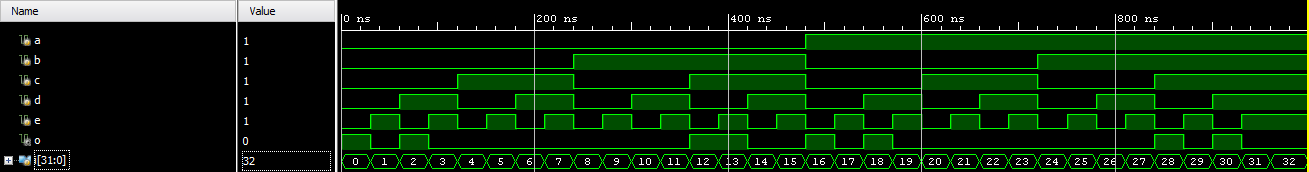
\includegraphics[width=\textwidth]{Images/waveform}
    \caption{The output of the obfuscated module.}
    \label{waveform1}
\end{figure}

Below are the results compiled from the waveform above.

\begin{table}[H]
    \centering
    \begin{tabular}{c | c | c | c | c || c}
    
        A & B & C & D & E & out \\ \hline \hline
        0 & 0 & 0 & 0 & 0 & 1 \\ \hline
        0 & 0 & 0 & 1 & 0 & 1 \\ \hline
        0 & 1 & 1 & 0 & 0 & 1 \\ \hline
        0 & 1 & 1 & 0 & 1 & 1 \\ \hline
        1 & 0 & 0 & 0 & 0 & 1 \\ \hline
        1 & 0 & 0 & 1 & 0 & 1 \\ \hline
        1 & 1 & 1 & 0 & 0 & 1 \\ \hline
        1 & 1 & 1 & 1 & 0 & 1 \\ \hline
        \multicolumn{5}{l}{Otherwise} & 0

    \end{tabular}
    \caption{Truth Table for obfuscated circuit.}
    \label{truthtable}
\end{table}

In short, there are eight different combinations of inputs
that result in a high output.

The following is a Karnaugh map simplification of the above
truth table. The different colors represent groupings of the
minterms: the four red bits are grouped together, the two
green bits are grouped together, and so on. Using the rules of
Karnaugh maps, this minimizes to the following Boolean function:
\begin{equation}
    \label{bool}
    f(A, B, C, D, E) =
    \bar{B}\bar{C}\bar{E} + ABC\bar{E} + \bar{A}BC\bar{D}
\end{equation}

\begin{figure}[H]
    \centering
    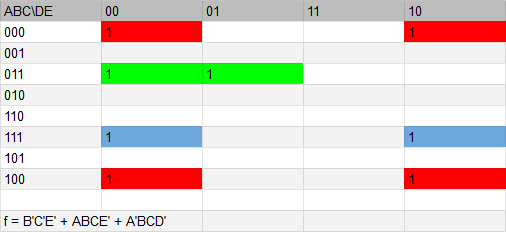
\includegraphics[width=\textwidth]{Images/kmap}
    \caption{Karnaugh map of truth table.}
    \label{kmap}
\end{figure}

\pagebreak

Making an equivalent circuit to reflect the given circuit
is as simple as making a module with Equation \ref{bool} inside it.
The following is a waveform with both the \c{original}
output (as shown in Figure \ref{waveform1}) and the
\c{equivalent} output from the equivalent circuit. Note how
their waveforms are the same.

\begin{figure}[H]
    \centering
    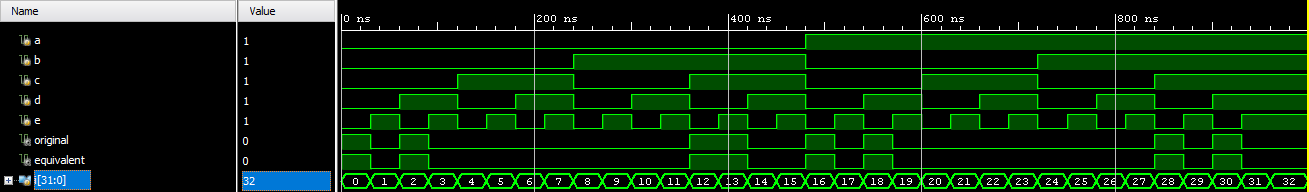
\includegraphics[width=\textwidth]{Images/waveform2}
    \caption{Waveform for both original and equivalent citcuits.}
    \label{waveform2}
\end{figure}

Lastly, I made a top-level module that drives the two
other modules with the same inputs, takes their outputs, and
XORs them together. Below is the waveform output of this module.
Note how the \c{eq} signal never goes high; it is not
satisfiable, and therefore the two circuits are equivalent.

\begin{figure}[H]
    \centering
    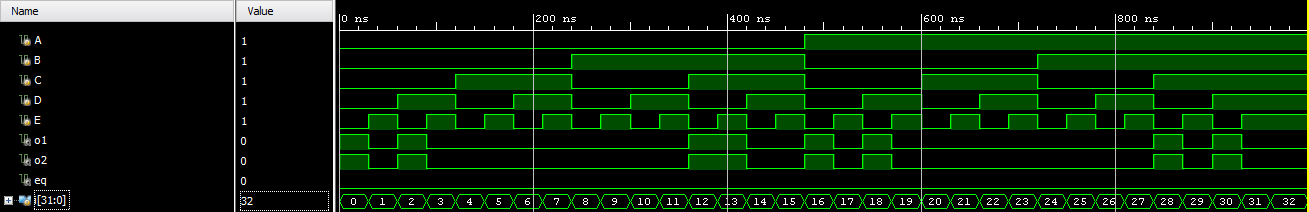
\includegraphics[width=\textwidth]{Images/waveform3}
    \caption{Waveform for top-level function.}
    \label{waveform3}
\end{figure}

Lastly, this was loaded onto the FPGA and tested for
compatibility with no flaws or issues.

\section{Media} Below are pictures of the board when the
original and equivalent circuits are on and off.

\begin{figure}[H]
    \centering
    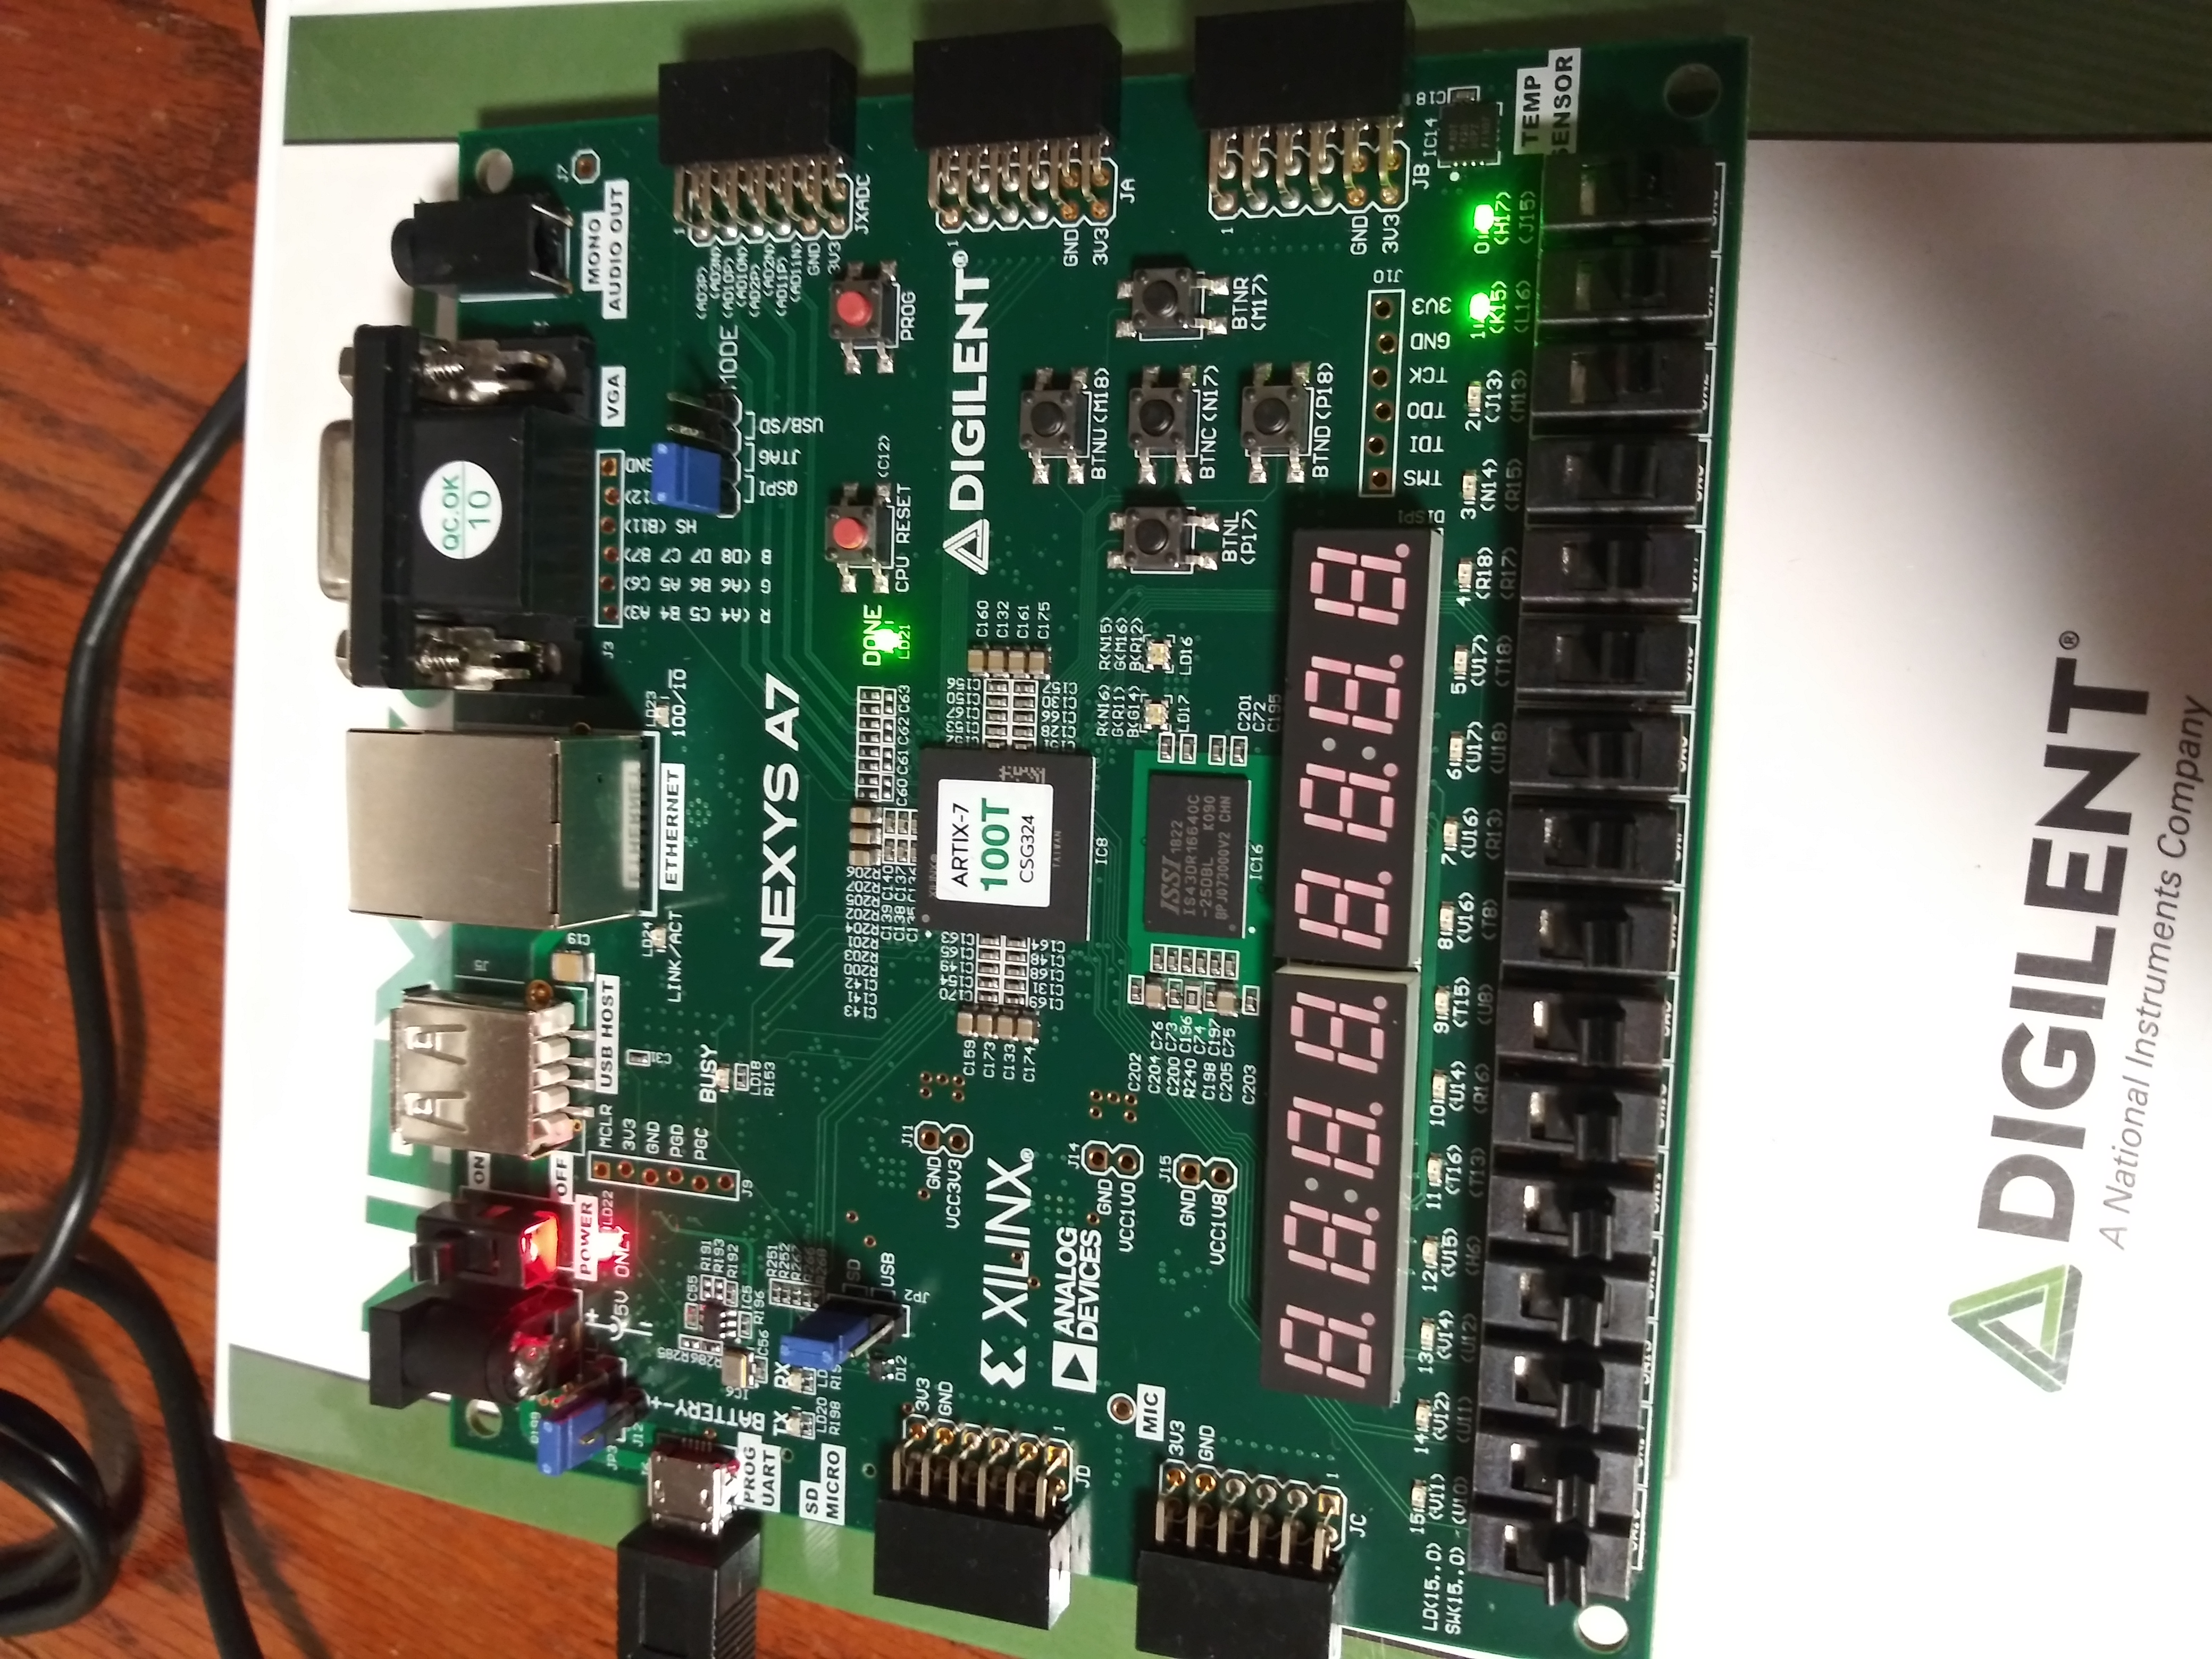
\includegraphics[width=\textwidth]{Images/board_on.jpg} 
    \caption{\c{\{a, b, c, d, e\} = 0}}
    \label{on}
\end{figure}
\begin{figure}[H]
    \centering
    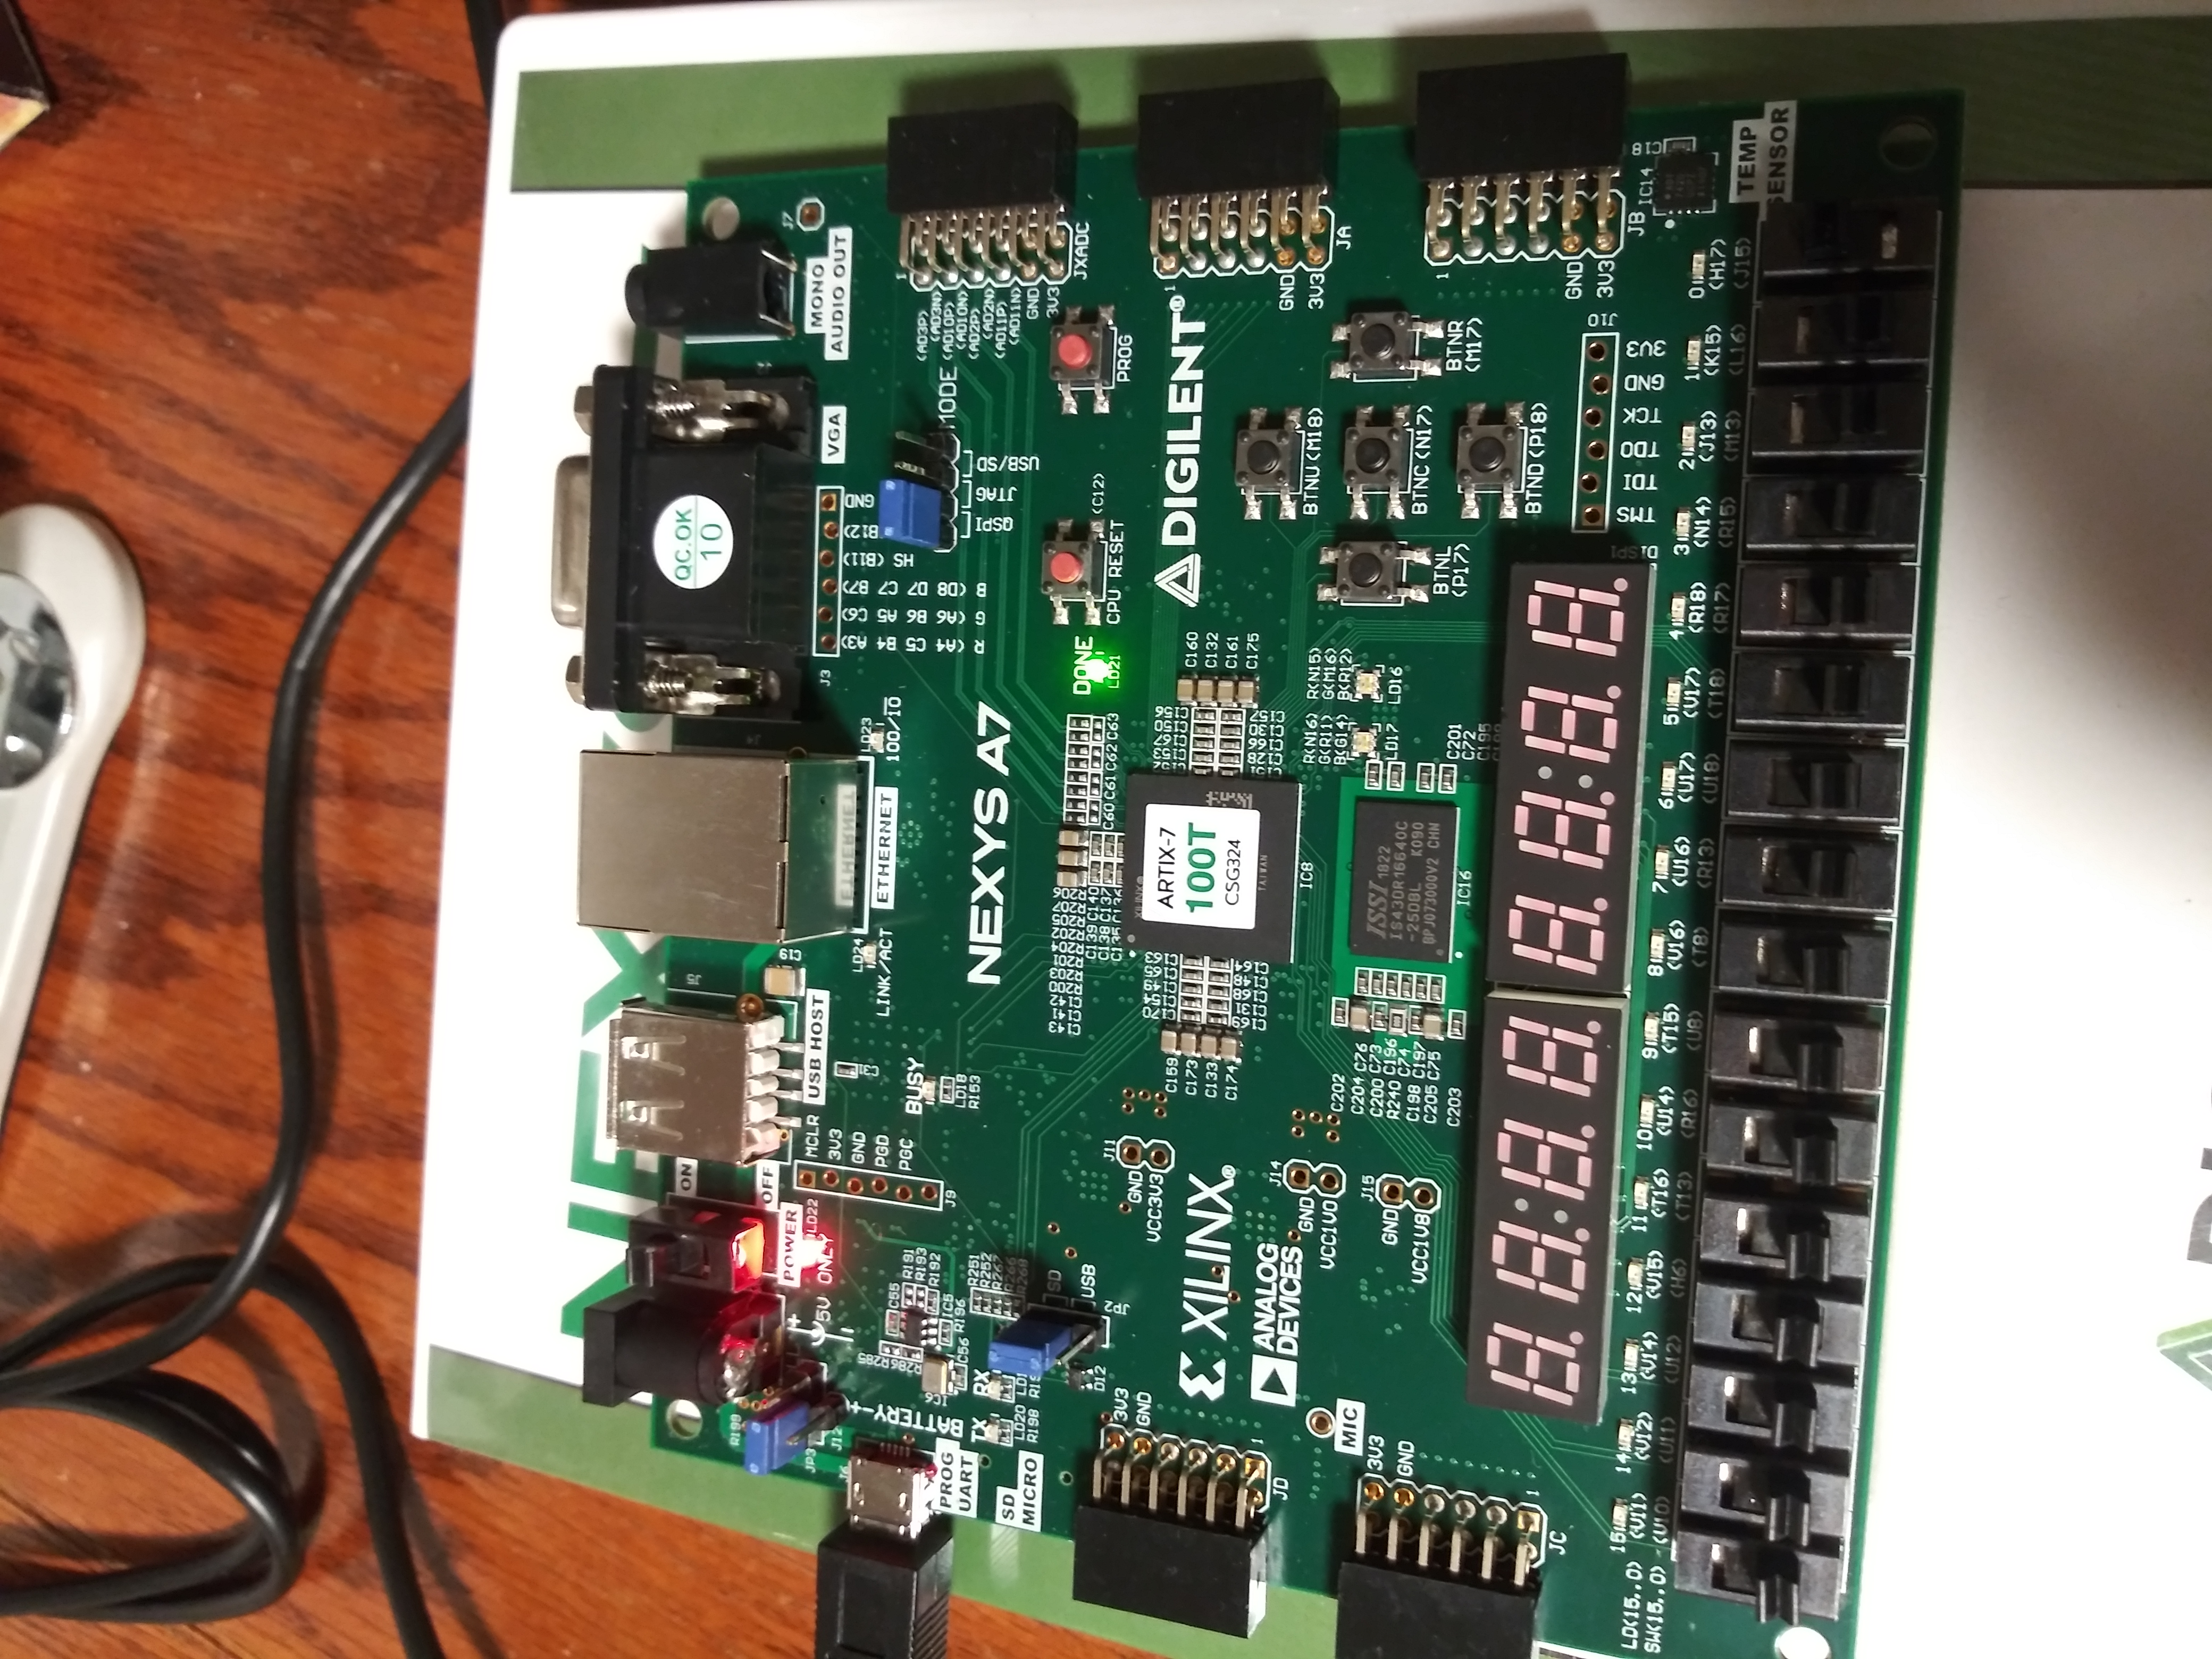
\includegraphics[width=\textwidth]{Images/board_off.jpg}
    \caption{\c{\{a, b, c, d, e\} = 1}}
    \label{off}
\end{figure}

\end{document}
